\documentclass{article}
\usepackage[utf8]{inputenc}
\usepackage[margin=1in]{geometry} % margins
\usepackage{listings} % in case we need to include source code
\usepackage{graphicx} % for pictures
\usepackage{float} % to put figures where they appear in source code
\usepackage{indentfirst} % indent first paragraph of section
\usepackage{pdfpages} % since the gui flowchart is a pdf
\DeclareGraphicsExtensions{.jpg,.JPG,.jpeg,.JPEG} % to detect jpg files
\DeclareGraphicsExtensions{.png,.PNG} % for png files

\usepackage{setspace} % so that we can do...
\doublespacing{} % this

\begin{document}

\noindent Nelson Batista

\noindent Abu Butt

\noindent Ichwan Palongengi

\noindent Adedamola Shomoye

\noindent Project 1 Progress Report

\noindent 4/21/2017

\section{GUI}

The GUI for the program has been implemented in the form of a website where users may create new reservations or view old ones. This website is hosted on a machine running Python Flask's built-in webserver, which is not too fancy, but suits our needs quite well. Flask displays pages by using ``templates'' along with its builtin template engine, Jinja. The intent of a template is to allow an outside program to combine the template with data, perhaps from a database or a previous POST request, into a complete webpage tailored to the provided data. 

For example, the template may have \texttt{\{\{ username \}\}} somewhere to display the username of the user viewing the page. Since this will, inevitably, depend on the specific user, the template is sent to the template engine along with the data, perhaps from a session cookie, necessary to replace \texttt{\{\{ username \}\}} with the literal username of the user through the Flask framework's \texttt{render\_template} function. The result is an HTML document tailored specifically for the user, which is then rendered by the user's browser.

Thus, using templates and a Python connector to a SQL database, we are able to send HTML pages reflecting data in the database.

In order to make a reservation, the passengers must enter their desired source and destination stations, using dropdown menus on the main page, as well as the time of day (morning, afternoon, evening), and of course the date of the trip. The user must also indicate whether it is to be a round trip, and if so they must specify the date and time of their intended return trip. This is submitted through an HTML form which takes the user to the ``search results'' page.

The ``search results'' page uses the data obtained from the POST request generated by submitting the form on the main page as arguments to a function used to query the databse for trains available under the parameters specified by the passenger. Specifically, the \texttt{get\_trains\_from\_station} function is called, which performs a SQL \texttt{select} statement to query the database for all trains which stop at both the source and destination stations at the time of day of the trip date. This returns a dictionary of train ids, which is then filtered using the \texttt{check\_free\_seats} function to get only those trains which have at least one seat free for every segment between the two stations. The \texttt{check\_free\_seats} function takes a start station and an end station along with a train id and trip date as arguments, and returns \texttt{true} if the train has at least one seat free for that date on every segment between the start and end stations. This is done using another, somewhat more complex \texttt{select} SQL statement. The set of trains returned by \texttt{get\_trains\_from\_station} is iterated over, and each train is appended to a \texttt{free\_trains} array only if \texttt{check\_free\_seats} returns \texttt{true} with that train's id supplied as an argument. The search results template then uses the \texttt{free\_trains} variable contents to display the trains available for the user to make reservations for.

On the search results page, the user may select any of the available trains to make a reservation for (or be told that there are no available trains). Upon reservation, we decrement the number of available free seats on the train for that date on every segment in between the start and end stations by 1, then write the new value back to the database.

This behavior and more is expressed in the flowchart on the following page.

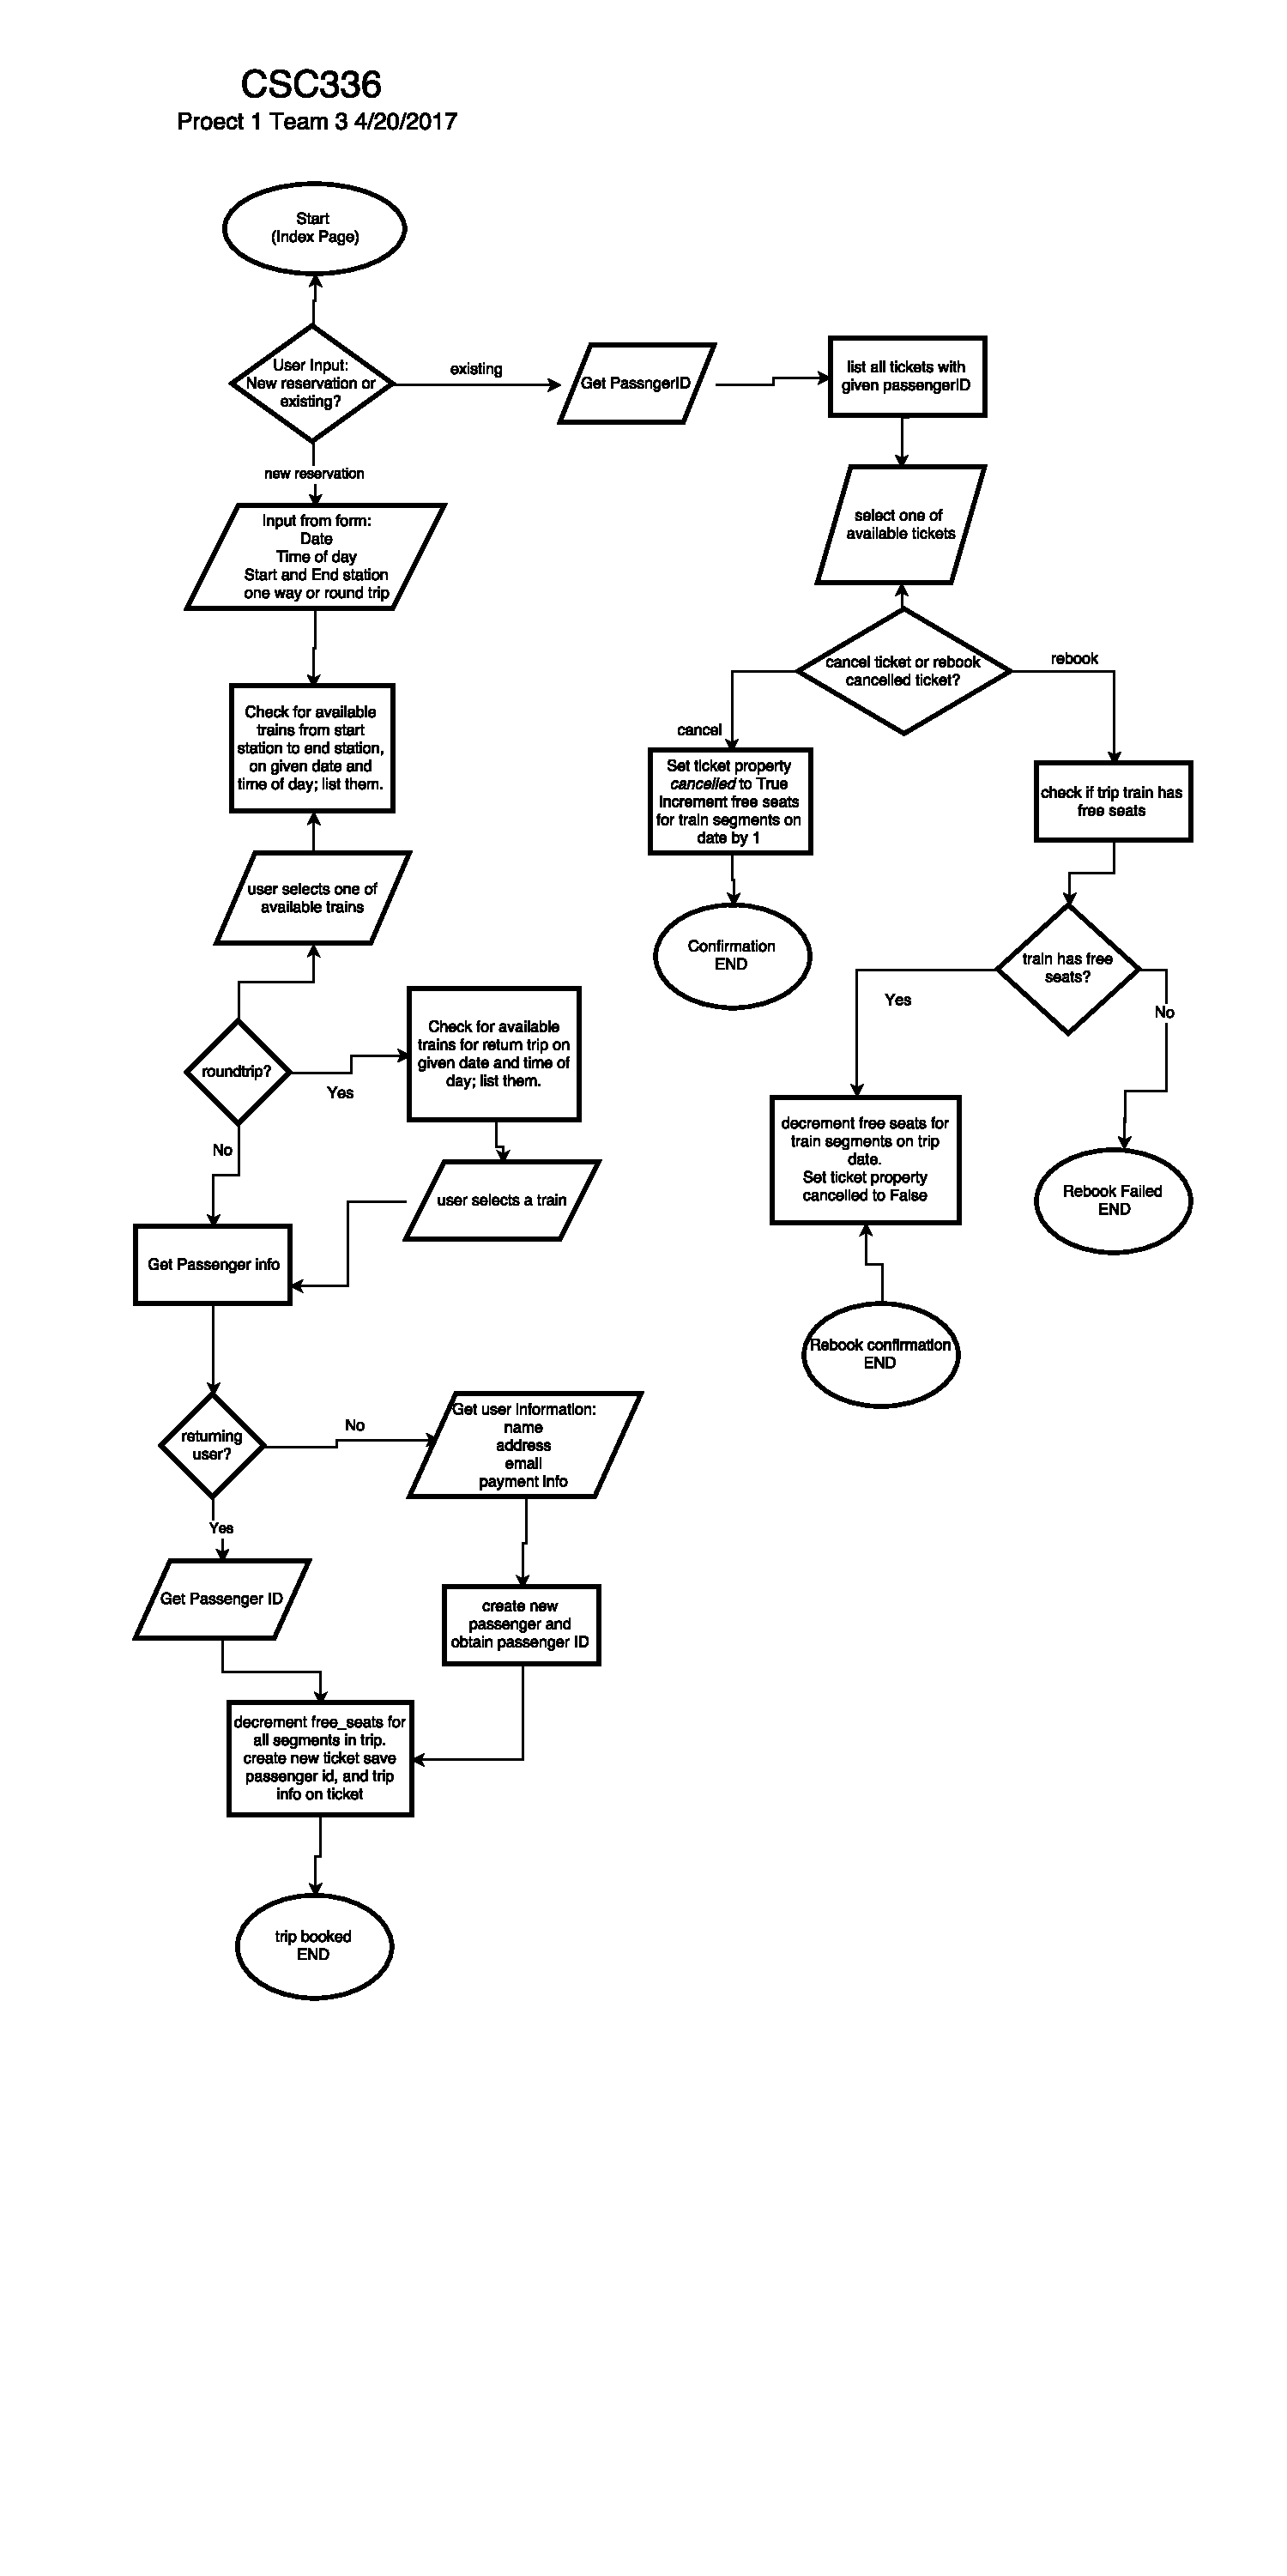
\includepdf[pages={-}]{336Team3BasicFlowChart.pdf}

\section{Database Layout}

The layout of the database itself is shown in the ER diagram provided alongside this report. First, we have the \texttt{Passengers} table, which contains a \texttt{passenger\_id} attribute, which serves as the primary key. Passengers purchase tickets, which represent reservations at certain times and dates, and which are themselves identified by the primary key \texttt{ticket\_id}. The \texttt{Tickets} table is related to the \texttt{Passengers} table by a foreign key which references \texttt{Passengers (passenger\_id)}.

All the relations, including foreign keys, are in the following Entity-Relation diagram:

\begin{figure}[H]
  \centering
  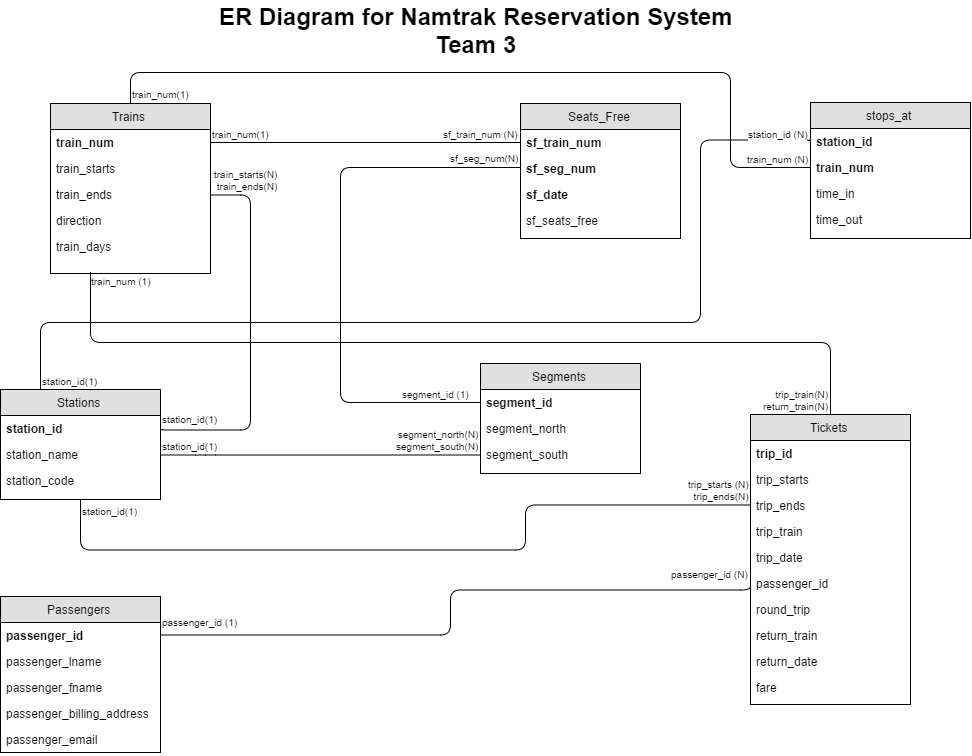
\includegraphics[scale=0.5]{erdiagram}
  \caption{ER Diagram for our database.}
\end{figure}

\end{document}

